%   Journal of Neural Engineering %

\pdfminorversion=4
\documentclass[10pt]{iopart}
\usepackage{graphicx}

\begin{document}

\title[Finding hidden functional states from EEG based on topological features]
        {Finding hidden functional states from EEG based on topological features}

\begin{abstract}

\noindent{\it Objective.}
The analysis of electroencephalograms (EEG) is primarily a manual, routine task performed exclusively by experts. Recent studies have addressed this issue and proposed the state-detecting algorithm (SDA) --- an automated technique to detect the functional stages with minimal human intervention. The method proved effective on recordings from Guhyasamaja meditation practice using spectral features. This article introduces an alternative approach to feature engineering for SDA--based on a novel field of topological data analysis (TDA). The applied methods aim to explore the spatial structure of the data, which is known to yield interesting, interpretable results when solving various problems.
\textit{Approach.}
We propose an algorithm to extract a comprehensive topological description of the EEG with almost 20,000 features and suggest QSDA --- a feature selection framework based on the performance of SDA\@. Then, we study the behavior of four typical dimensionality reduction techniques and employ information value analysis (IV) to explore the significance of the features. Finally, we detect the brain regions that produce the most valuable data for the task based on IV and QSDA scores.
\textit{Main results.}
We applied the approach to the EEG recordings of the meditation practice performed by 30 Tibetan monks and thoroughly analyzed the first 3. The proposed method yielded well-separated stage boundaries for all subjects, suggesting that TDA complements the spectral features and reveals new, previously unknown patterns. Moreover, QSDA effectively filtered out the noisy features and appeared consistent with the IV\@. Finally, the approach was confirmed statistically stable, showing poor quality when applied to randomly shuffled epochs.
\textit{Significance.}
The study proves the existence of significant patterns in the spatial structure of the EEG, which may have interesting physiological interpretations leading to more effective and robust functional stage detection. The proposed feature selection framework appeared practical and may apply to other features.

\end{abstract}

\vspace{2pc}
\noindent{\it Keywords\/}: EEG, topological data analysis, state-detecting algorithm, functional states, feature selection

\submitto{\JNE}

\ioptwocol{}

\section{Introduction}

EEG signals are a powerful tool for studying human brain activity and diagnosing numerous diseases and abnormalities. However, its analysis is usually performed manually, and automation in the field is vastly limited to particular tasks. Most algorithms rely on information about events artificially created during the experiment (external interactions with the subject, reactions, responses, etc.). Nowadays, the study of EEG of continuous processes that do not allow external interactions with the subject is of significant value for neurophysiology, including somnology and epilepsy detection.

One such task is finding the boundaries of functional states in the EEG that split the recording into well-separable parts denoting the occurrence of some naturally induced events at that time. To solve this, \cite{SDA} recently presented the SDA, which solves the problem without additional information about the events that occurred during the experiment (including their quantity) using traditional data clustering methods. The technique consists of two principal stages:
\begin{enumerate}
    \item
        Find the potential boundaries of functional states for different values of hyperparameters using a hierarchical clustering algorithm that supports a connectivity constraint;
    \item
        Apply a suitable clustering technique to the sets of potential answers obtained in the first stage and select the final boundaries that achieve the best clustering quality.
\end{enumerate}


To use the algorithm, one should clean and preprocess the EEG data, split it into time epochs, and embed the corresponding time series into some feature space. As shown in the original work, the method demonstrates good quality for EEG obtained from the meditation of Buddhist monks using the Tantric Guhyasamaja practice when extracting the traditional spectral features to describe the time series --- PSD, PLV, and Coherence.

However, these features mostly describe the frequencies and correlations in the time series, leaving significant portions of information presented in the EEG signals unexplored. Nowadays, there is ongoing research on the applications of another modern approach to feature extraction --- topological data analysis (TDA), which identifies the relationships in the data by studying its geometry and spatial structure via the research of the appearance and disappearance of holes and voids in the data across different dimensions. It allows for the quantification of different structural characteristics of the signal, which are known to be more convenient for some problems, including in physiology, can achieve better quality, and the results may be relatively easy to interpret.

Numerous recent studies show that TDA demonstrates high quality in solving various problems, including time series and EEG in particular. For example, \cite{chazal2024topologicalanalysisdetectinganomalies,rai2024identifyingextremeeventsstock,heo2024persistenthomologyfeaturedtime,chrétien2024timetopologicalanalysiseeg} present numerous theoretically guaranteed approaches to detecting anomalies in multivariate time series, demonstrating their quality with diverse datasets ranging from synthetic, generated ones to real-world examples, including the stock market, music recordings, and epilepsy detection. \cite{dimontesano2024dynamicallymaintainingpersistenthomology} proposes a data structure to maintain and recalculate the persistent homology as the epochs are added to or removed from the time series, and \cite{ost2024bananatreespersistencetime} elaborates on the real-world applications of the technique.  \cite{cai2024topologicalfeaturesearchmethod} demonstrates the applications of TDA in ADHD classification, achieving exceptional results on typical datasets in the field with high precision and robustness. Finally, \cite{deng2024twostagehierarchicalexplainablefeature} suggests a TDA-based feature selection framework to improve the performance of dimensionality reduction in sleep stage classification.

In this study, we apply the topological data analysis to find the functional states in the EEG of a continuous process --- the aforementioned Tantric Guhyasamaja meditation practice performed by 30 Buddhist monks. To estimate its applicability to the problem, we calculate a comprehensive description of almost 20,000 features retrieved from different aspects of the time series with diverse topological methods and statistical characteristics. We also present an SDA-based feature selection framework to determine a reasonable number of features (1,500 -- 2,000) that allegedly achieve the best quality of the final answer. Moreover, we evaluate the performance of typical dimensionality reduction techniques (PCA, UMAP, AE, RTD AE) to further decrease the number of components up to 15. Then, we compare the final state boundaries computed from different features (traditional, topological, or both combined) and draw conclusions based on the output's quality metrics. Finally, we utilize the information value analysis to estimate the influence of individual features on the answer, confirm the stability of our feature selection algorithm, and reinforce the obtained results. Additionally, to ensure the statistical significance of the approach, we repeat the study for the EEG obtained by shuffling the epochs of the original data, expecting SDA to detect no good boundaries.

For debugging purposes and hyperparameter selection, we used only the EEG recording of object 1. The validation dataset comprised the data from objects 2 and 3, which were also thoroughly investigated in the study. Finally, the remaining 27 recordings were utilized as a final control to verify the results on a larger set. 

\section{Dataset}

In the study, we used the data collected and preprocessed in the original article~\cite{SDA}. This section provides a brief description of the methods used.

\subsection{Data collection}

Guhyasamaja Tantra is a traditional meditation practice that follows the strict principles enshrined in the sacred scriptures of Buddhism. Its essential part consists of 8 subsequent stages, the duration of which may vary in different versions.

The data used in the study is the EEG recordings of the successful meditation of 30 Tibetan Buddhist monks practicing Guhyasamaja Tantra for many decades. The first three are referred to in this study as object 1, object 2, and object 3, respectively. The signals were acquired using an NVX-52 system at a 500 Hz sampling rate with analog bandpass filtering from 0.1 to 200 Hz and a digital notch filter at 50 Hz to remove the power line noise. As a result, for objects~1 3, the recordings lasting 935, 2344, and 1302 seconds were obtained.

\subsection{Data preprocessing}

The following data preprocessing was performed with Python using the MNE library~\cite{MNE}. Several procedures, including a bandpass filter at frequencies of 0.9 -- 40 Hz and independent component analysis, were applied to remove artifacts unrelated to the process of interest (respiratory and muscle activity, eye blinking, heartbeat, etc.). The recordings were then divided into 1-second epochs, 10 -- 15\% of which, most deviating from the average by the power spectral density, were removed. No overlap was used when creating the epochs except for object 1, where an overlap of 0.2 seconds was adopted to increase the amount of available data for the study. The resulting data for objects~1 3 is the arrays of 1046, 2019, and 1180 epochs, respectively, where each epoch is a multidimensional time series described by a $38\times501$ matrix. Each of the 38 channels corresponds to one of the electrodes used during the experiment.

For ease of analysis, similar to the original article, the electrodes were divided into 17 groups according to the parts of the brain they recorded, as shown in \fref{figure1}: pre-frontal (Fp1, Fp2, Fpz), left frontal (F3, F7, FC3, FT7), midline frontal (Fz, FCz), right frontal (F4, F8, FC4, FT8), left central (C3, CP3), midline central (Cz, CPz), right central (C4, CP4), left temporal (T3, T5, TP7), right temporal (T4, T6, TP8), left parietal (P3, P5), middle parietal (Pz), right parietal (P4, P6), left occipital (PO3, PO7, O1), middle occipital (POz, Oz), right occipital (PO4, PO8, O2), and two ear electrodes A1 (left) and A2 (right). However, the ear electrodes were excluded from the recordings as their data primarily describes muscular activity, which is not interesting to the study.

\begin{figure}
    \centering
    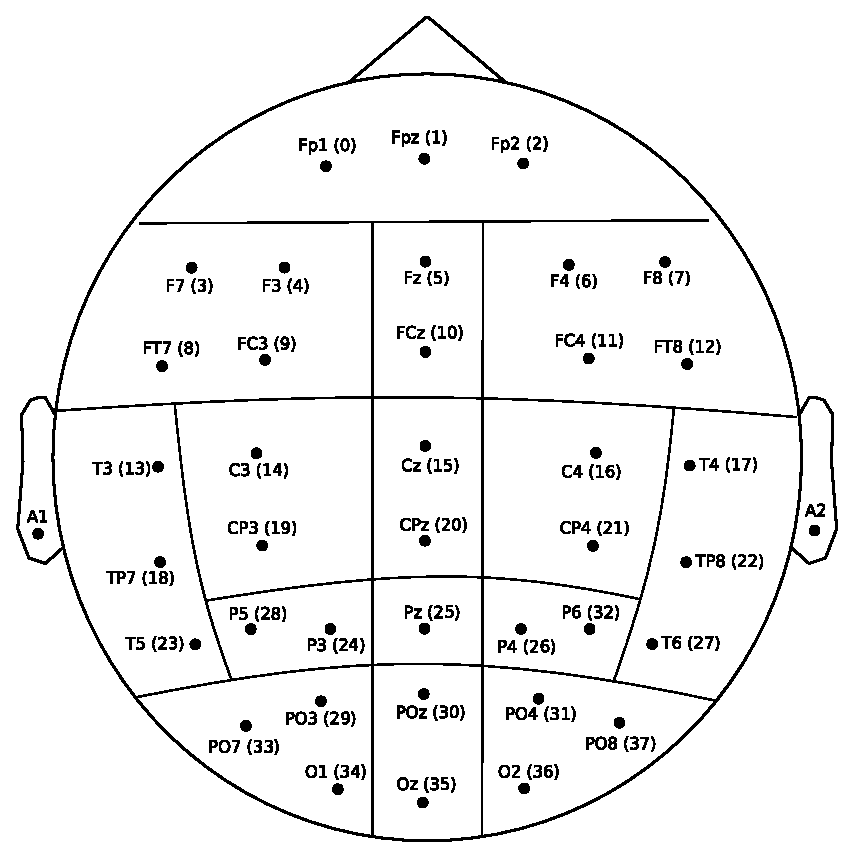
\includegraphics[width=0.66 \columnwidth]{figure1.eps}
    \caption{Location of electrodes during the experiment and their division into groups.}
    \label{figure1}
\end{figure}

\section{State-Detecting algorithm}

The State-Detecting algorithm is a novel data-driven approach to finding the functional states in the EEG from its feature description --- a matrix that maps each epoch to a feature vector of a given dimension. The technique combines two clustering methods to find the resulting edges accounting for the continuity of the process under analysis in time. Here, we briefly review the general principles of both stages. Please refer to the original work~\cite{SDA} for a more detailed description.

In the first step, the algorithm finds the potential boundaries of functional states using Ward's hierarchical clustering method with different values of the number of sought stages and the maximum time between epochs in the connectivity matrix. Then, the obtained boundaries are sorted, and the neighboring stages are merged if they are too short or do not differ enough by the Ward distance.

During the second step, the algorithm utilizes K-Means to select the candidates for the final boundaries of functional states based on the results of the first step. For this, SDA applies the mentioned clustering method to the joint sets of potential boundaries obtained previously to determine the required number of stages. Finally, the algorithm computes the resulting boundaries as modes and medians of the obtained clusters merged similarly to the first stage to guarantee their sufficient length and dissimilarity.

The conclusive answer is decided by an expert decision accounting for the clustering quality metrics: the Ward's and centroid distances, the silhouette coefficient, the Calinski--Harabasz index, and the Davies--Bouldin index. In this study, we primarily focused on the silhouette coefficient that is calculated for one object using equation \eref{eq1} and shows how similar this object is to other objects in its cluster ($C_x$) in comparison with objects in different clusters ($C_y$). The single value for the entire set is obtained by averaging the results across all studied objects. The metric value ranges from -1 to 1, where positive values indicate that the object is assigned to the correct cluster, which is well separated from other clusters.
\begin{eqnarray}
    a(x, C_x) = {(|C_x| - 1)} ^ {-1} \sum_{y \in C_x} ||x - y||, \nonumber\\
    b(x, C_x) = \min_{C_y \ne C_x} {|C_y|} ^ {-1} \sum_{y \in C_y} ||x - y||, \nonumber\\
    s(x, C_x) = (b - a)~~/~~\max(a, b), \label{eq1}
\end{eqnarray}

\section{Topological data analysis}

Topological data analysis is a modern approach to analyzing different kinds of data by reducing their dimensionality without significant loss of information by studying the spatial characteristics (shape, structure, etc.) using algebraic topology. The main tools of this approach are persistent homologies and persistence diagrams, calculated for metric spaces to describe the number and stability of multidimensional `holes' in them. It has been proven that minor perturbations in the source data do not have significant effects on the results, which makes it possible to use the information contained in the diagrams to solve various machine-learning problems according to the following general principle:

\begin{enumerate}
    \item
        Transform the input data into a metric space --- a set of points with a correctly defined distance function. For the time series, we utilized two principal approaches:

        \begin{enumerate}
            \item
                Studying the behavior of distinct components of both univariate and multivariate time series with the Takens' embedding algorithm~\cite{10.1007/BFb0091924,perea2013slidingwindowspersistenceapplication}. The general ways to select the algorithm's hyperparameters (that is, the dimensionality of the embeddings~\cite{PhysRevA.45.3403} and the time delays between them~\cite{PhysRevA.33.1134}) aim to optimize the number of false-neighboring pairs of points and the mutual information.
            \item 
                Examining the correlations between the components of a multivariate time series by defining the distances between them with the Pearson dissimilarity.
        \end{enumerate}

    \item 
        Construct a sequence of nested simplicial complexes --- topological spaces homotopy equivalent to the unions of the balls of a given radius around the points from a given set for all positive values of the filtration parameter. The Nerve theorem~\cite{Borsuk1948} guarantees that the \v{C}ech complex~\cite{Cech1932}, containing the simplices for which the set of balls of a given radius around the vertices has a non-empty intersection, satisfies this property. However, its construction is computationally expensive, which makes the structure impractical. Instead, we used the approximation of the \v{C}ech complex called the Vietoris--Rips complex~\cite{Vietoris1927}, which does not satisfy the required property in general but is sufficient for most practical problems. The structure represents the unions of simple geometric figures of various dimensions (segments, triangles, tetrahedrons, etc.), called simplices, for which all pairwise distances between vertices do not exceed the filtration parameter. The general algorithm to construct these structures is to observe the appearance and disappearance of simplices with increasing $\epsilon$, although several more efficient algorithms have been proposed \cite{ZOMORODIAN2010263,rieser2024newconstructionvietorisripscomplex,Bauer_2021}. \Fref{figure2} shows the examples of \v{C}ech and Vietoris--Rips complexes for a synthetic point cloud.
        \begin{figure}
            \centering
            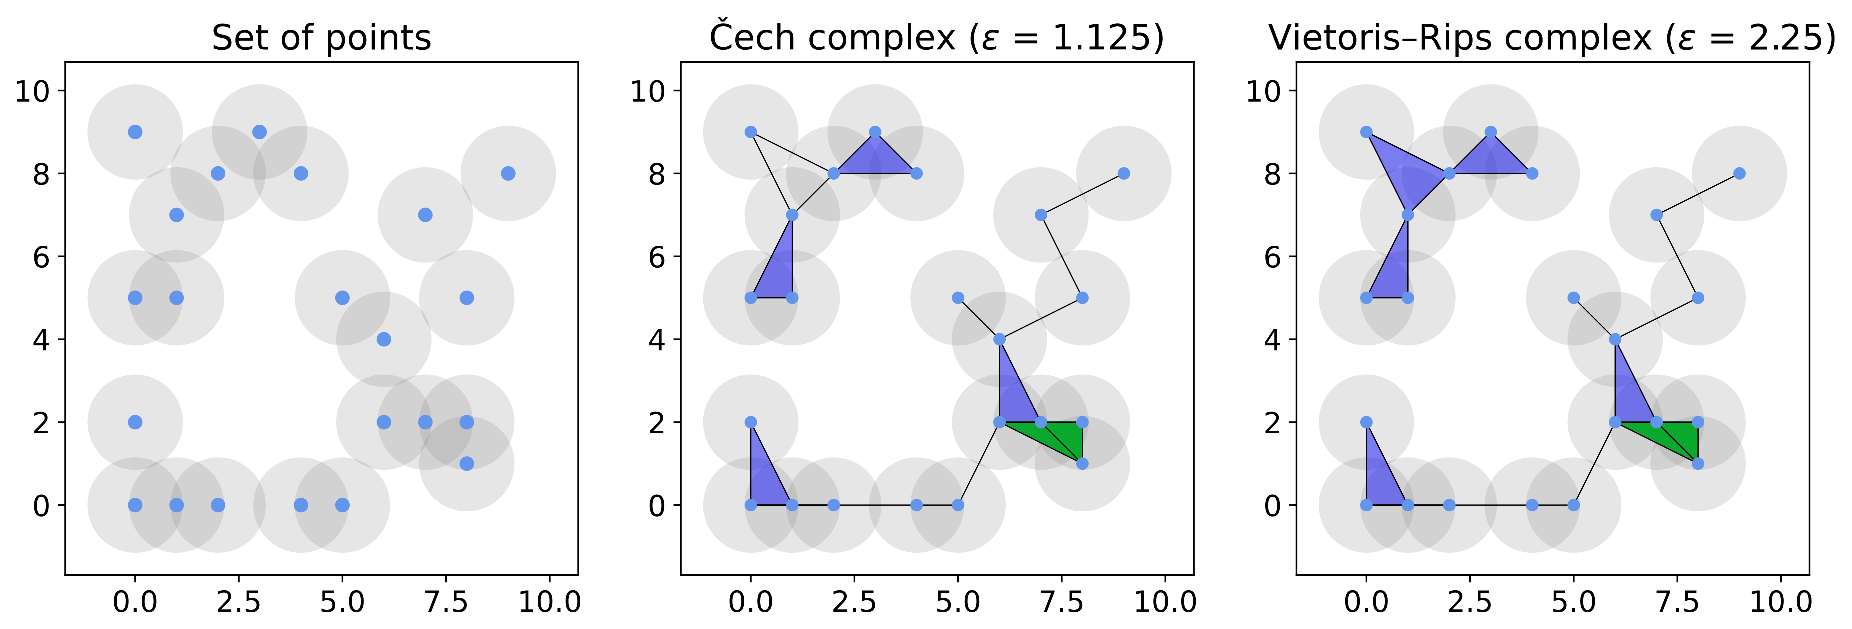
\includegraphics[width=\columnwidth]{figure2.eps}
            \caption{A synthetic point cloud with its \v{C}ech and Vietoris--Rips complexes for some values of the filtration parameter.}
            \label{figure2}
        \end{figure}\

    \item 
        Calculate the persistent homology of the resulting structure based on the `times' of appearance and disappearance of simplices. Construct and filter (that is, remove the points closest to the diagonal, which carry little information and most likely describe the `noise' in the data) the persistence diagram where each simplex corresponds to one point with coordinates along the `x' and `y' axes equal to the moments of its appearance in and disappearance from the complex, respectively.

    \item 
        Extract the features --- various topological and statistical characteristics --- from the persistence diagram. The principal approach studies the Betti numbers~\cite{Zomorodian2005} representing the maximum amount of cuts before separating the surface into two parts. One can also prove that the k-th Betti number equals the quantity of k-dimensional `holes' in the original metric space, which, in turn, is equivalent to the number of simplices of dimension k. Multiple other techniques have been proposed, including the persistence entropy~\cite{10.1007/978-3-319-29228-1_11}, landscape~\cite{bubenik2015statisticaltopologicaldataanalysis}, silhouette~\cite{chazal2013stochasticconvergencepersistencelandscapes}, and amplitude. The latter is particularly interesting as a measure of the difference between a given persistence diagram and an `empty' diagram, computed based on other topological characteristics as well as methods from adjacent fields of study~\cite{kerber2016geometryhelpscomparepersistence}, such as the Wasserstein~\cite{10.1145/62212.62253} and bottleneck distance~\cite{Efrat2001}. These features have proved effective for many classical machine learning algorithms solving various problems.

    \item 
        Select the most valuable features and reduce the dimensionality of the obtained feature space to remove the noise and improve the performance of machine learning algorithms applied later. For this, we used two predominant traditional techniques --- the principal component analysis~\cite{Eckart_Young_1936} (PCA) and the autoencoder~\cite{Autoencoder} (AE) --- as well as two topology-based methods --- the uniform manifold approximation and projection~\cite{mcinnes2020umapuniformmanifoldapproximation} (UMAP) and the representation topology divergence autoencoder~\cite{trofimov2023learningtopologypreservingdatarepresentations} (RTD AE).
\end{enumerate}

\section{Feature engineering}

As shown in \fref{figure3}, we employed three independent techniques to extract features from the EEG.\@

First, the EEG components are processed independently to analyze the records obtained at each electrode separately from other parameters. For this, we divide the epochs --- multidimensional time series --- into sets of one-dimensional time series, each corresponding to one electrode during the experiment. Then, we calculate the optimal hyperparameters of the Takens embedding algorithm for each obtained time series. As a result, we acquire a set of hyperparameters for each epoch of each EEG component and select one value for each of them that is optimal for most epochs. Finally, we transform the original EEG into metric spaces using the Takens algorithm with the calculated best hyperparameters, construct the Vietoris--Rips complexes, and compute the persistence diagrams.

This approach describes the individual EEG variables and detects most of the significant patterns in the data. However, it does not account for the correlations between the components of the time series, which may contain the information necessary to solve the problem.

To address this issue, the second approach aims to analyze the relationships between EEG components. The point clouds are obtained by calculating the Pearson dissimilarities between the channels for each epoch and all its sliding windows of a given size with a fixed step. The result is a set of matrices describing the metric spaces consisting of 38 points, with distances reflecting the correlations between the corresponding components of the time series. Then, similar to other techniques, we apply the Vietoris--Rips complexes to construct the persistence diagrams and obtain the feature descriptions of the EEG.\@

Eventually, we analyze the time series as a whole without explicitly focusing on specific characteristics. To do this, we employ the multidimensional Takens embedding algorithm with hyperparameters determined experimentally but kept identical for all components. The retrieved metric spaces are again processed with Vietoris--Rips complexes to obtain the resulting features.

\begin{figure}
    \centering
    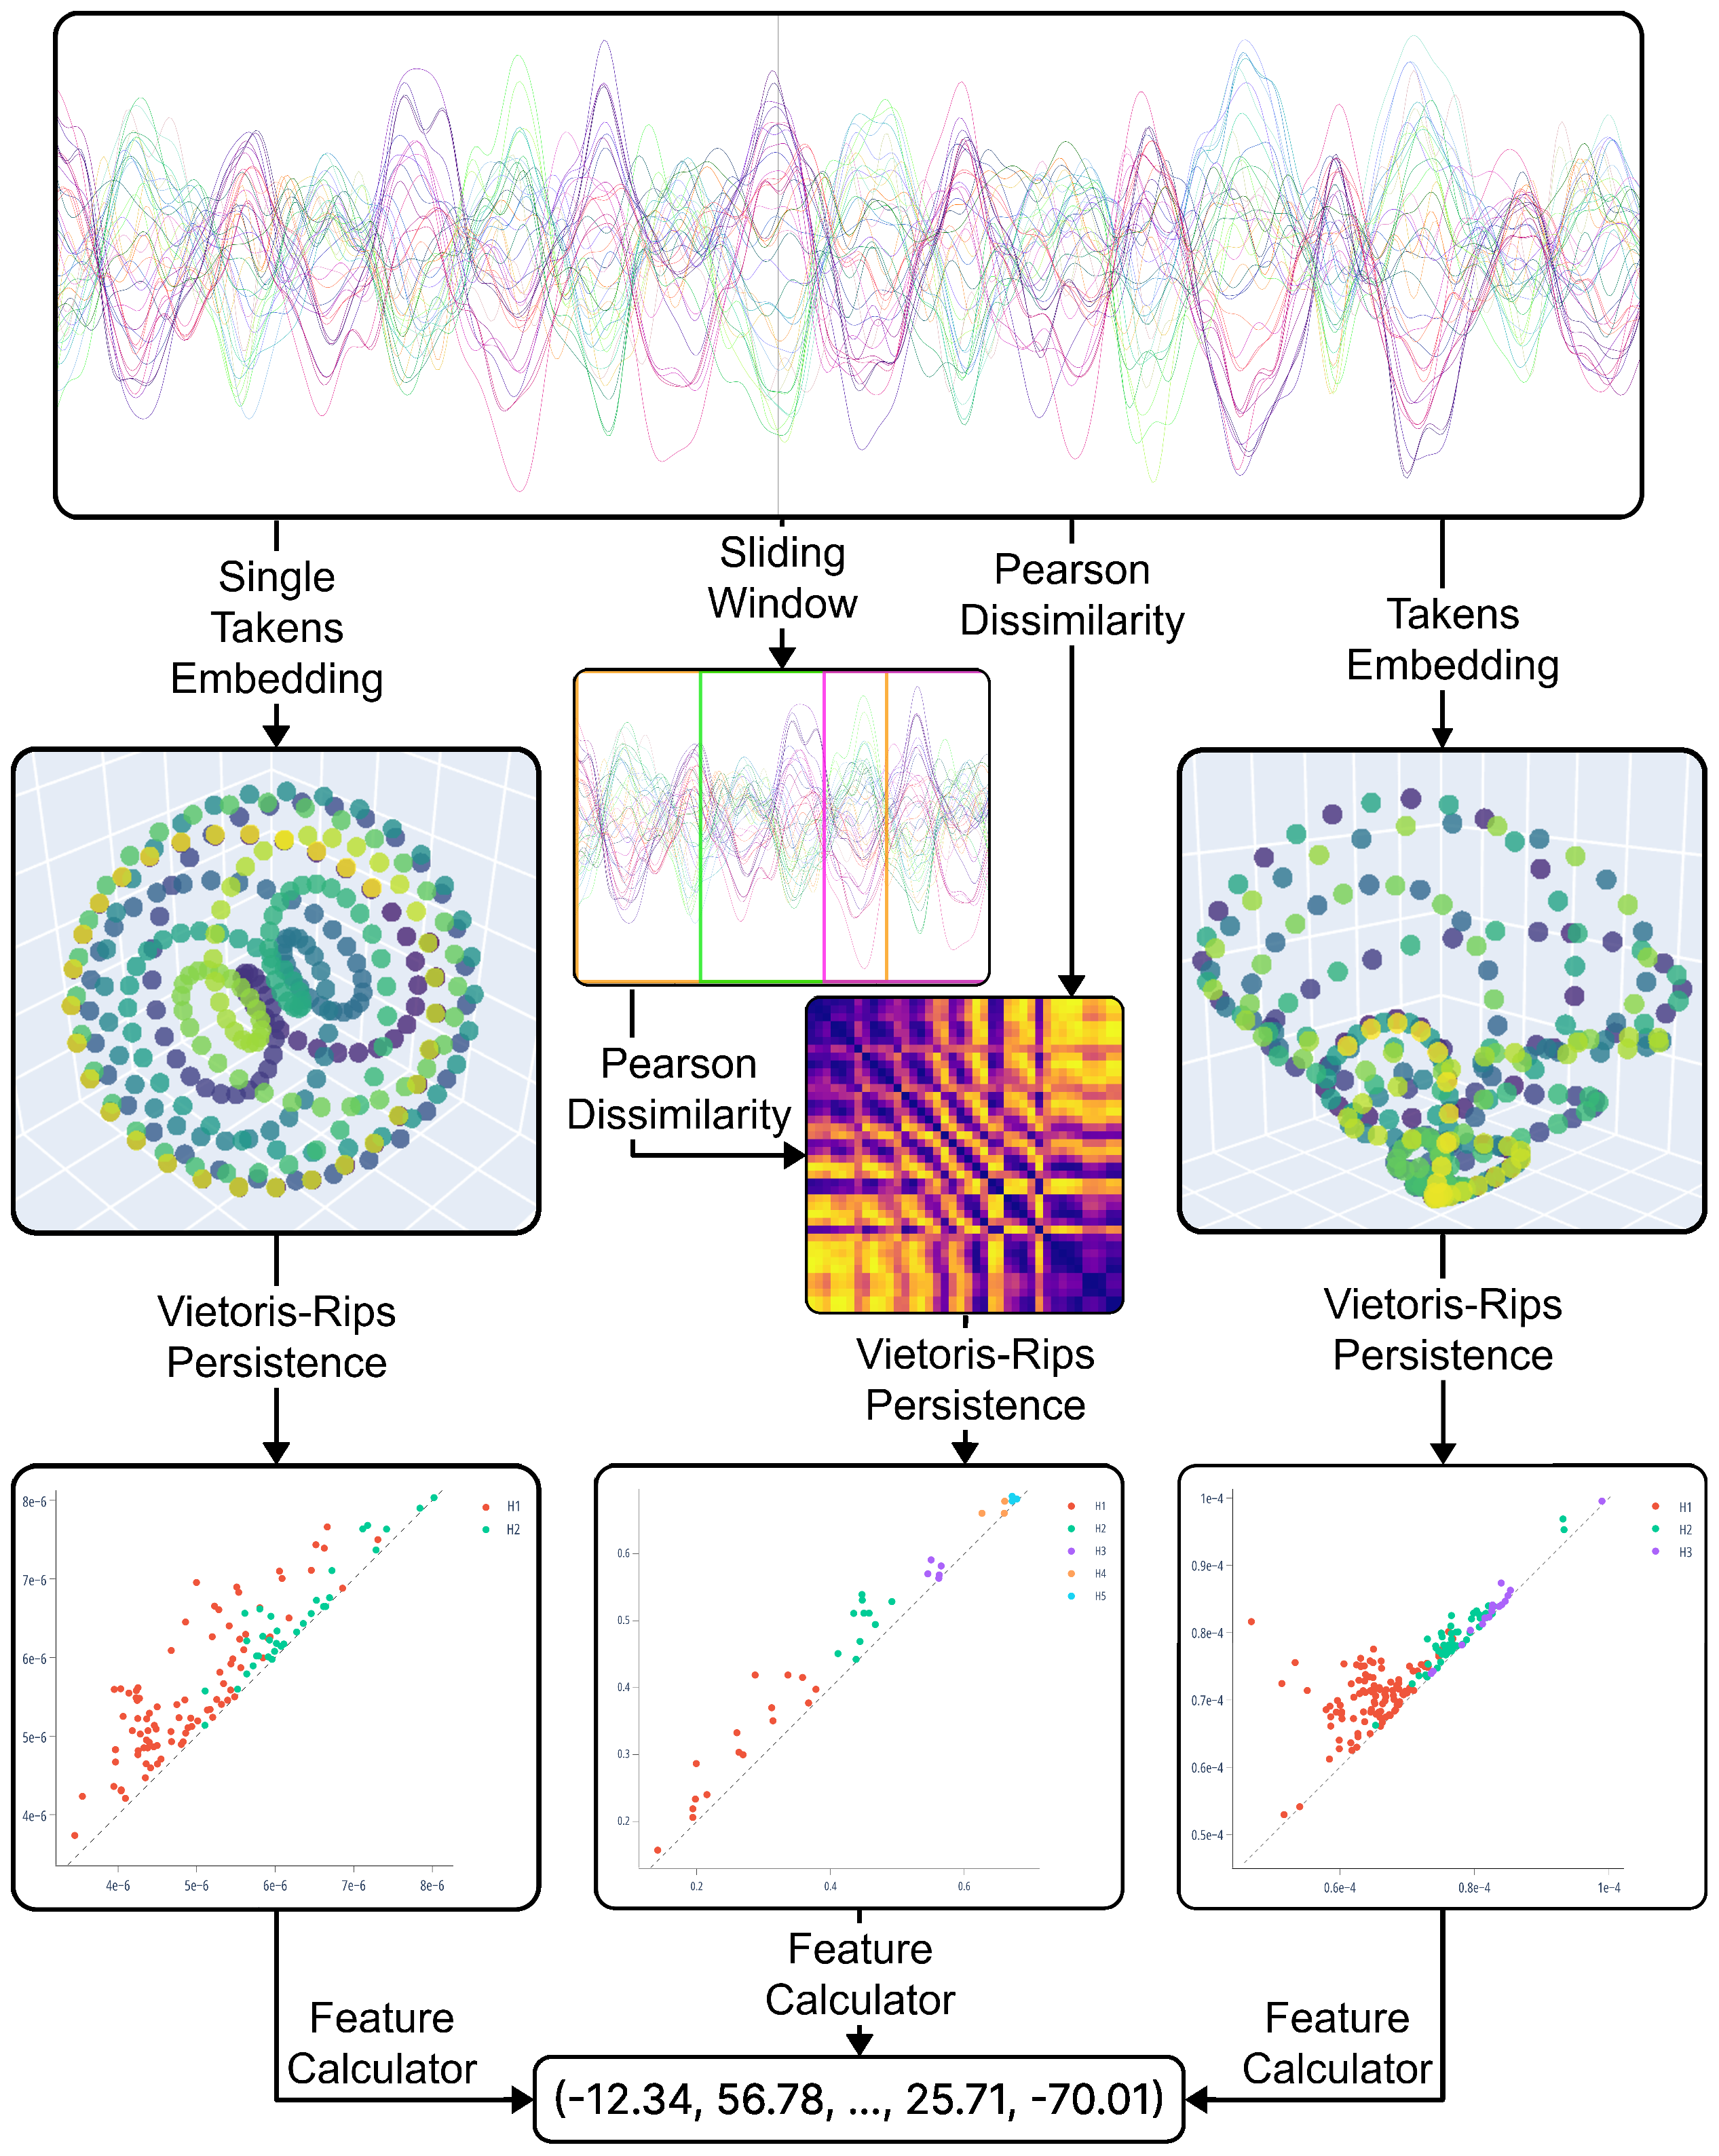
\includegraphics[width=\columnwidth]{figure3.eps}
    \caption{The scheme of the algorithm for extracting the topological features from the EEG.\@}
    \label{figure3}
\end{figure}

\subsection{Extracting features from persistence diagrams}

To vectorize the persistence diagrams as part of the feature engineering process, we implemented the pipeline presented in \fref{figure4}, which extracts feature descriptions from persistence diagrams.

\begin{figure}
    \centering
    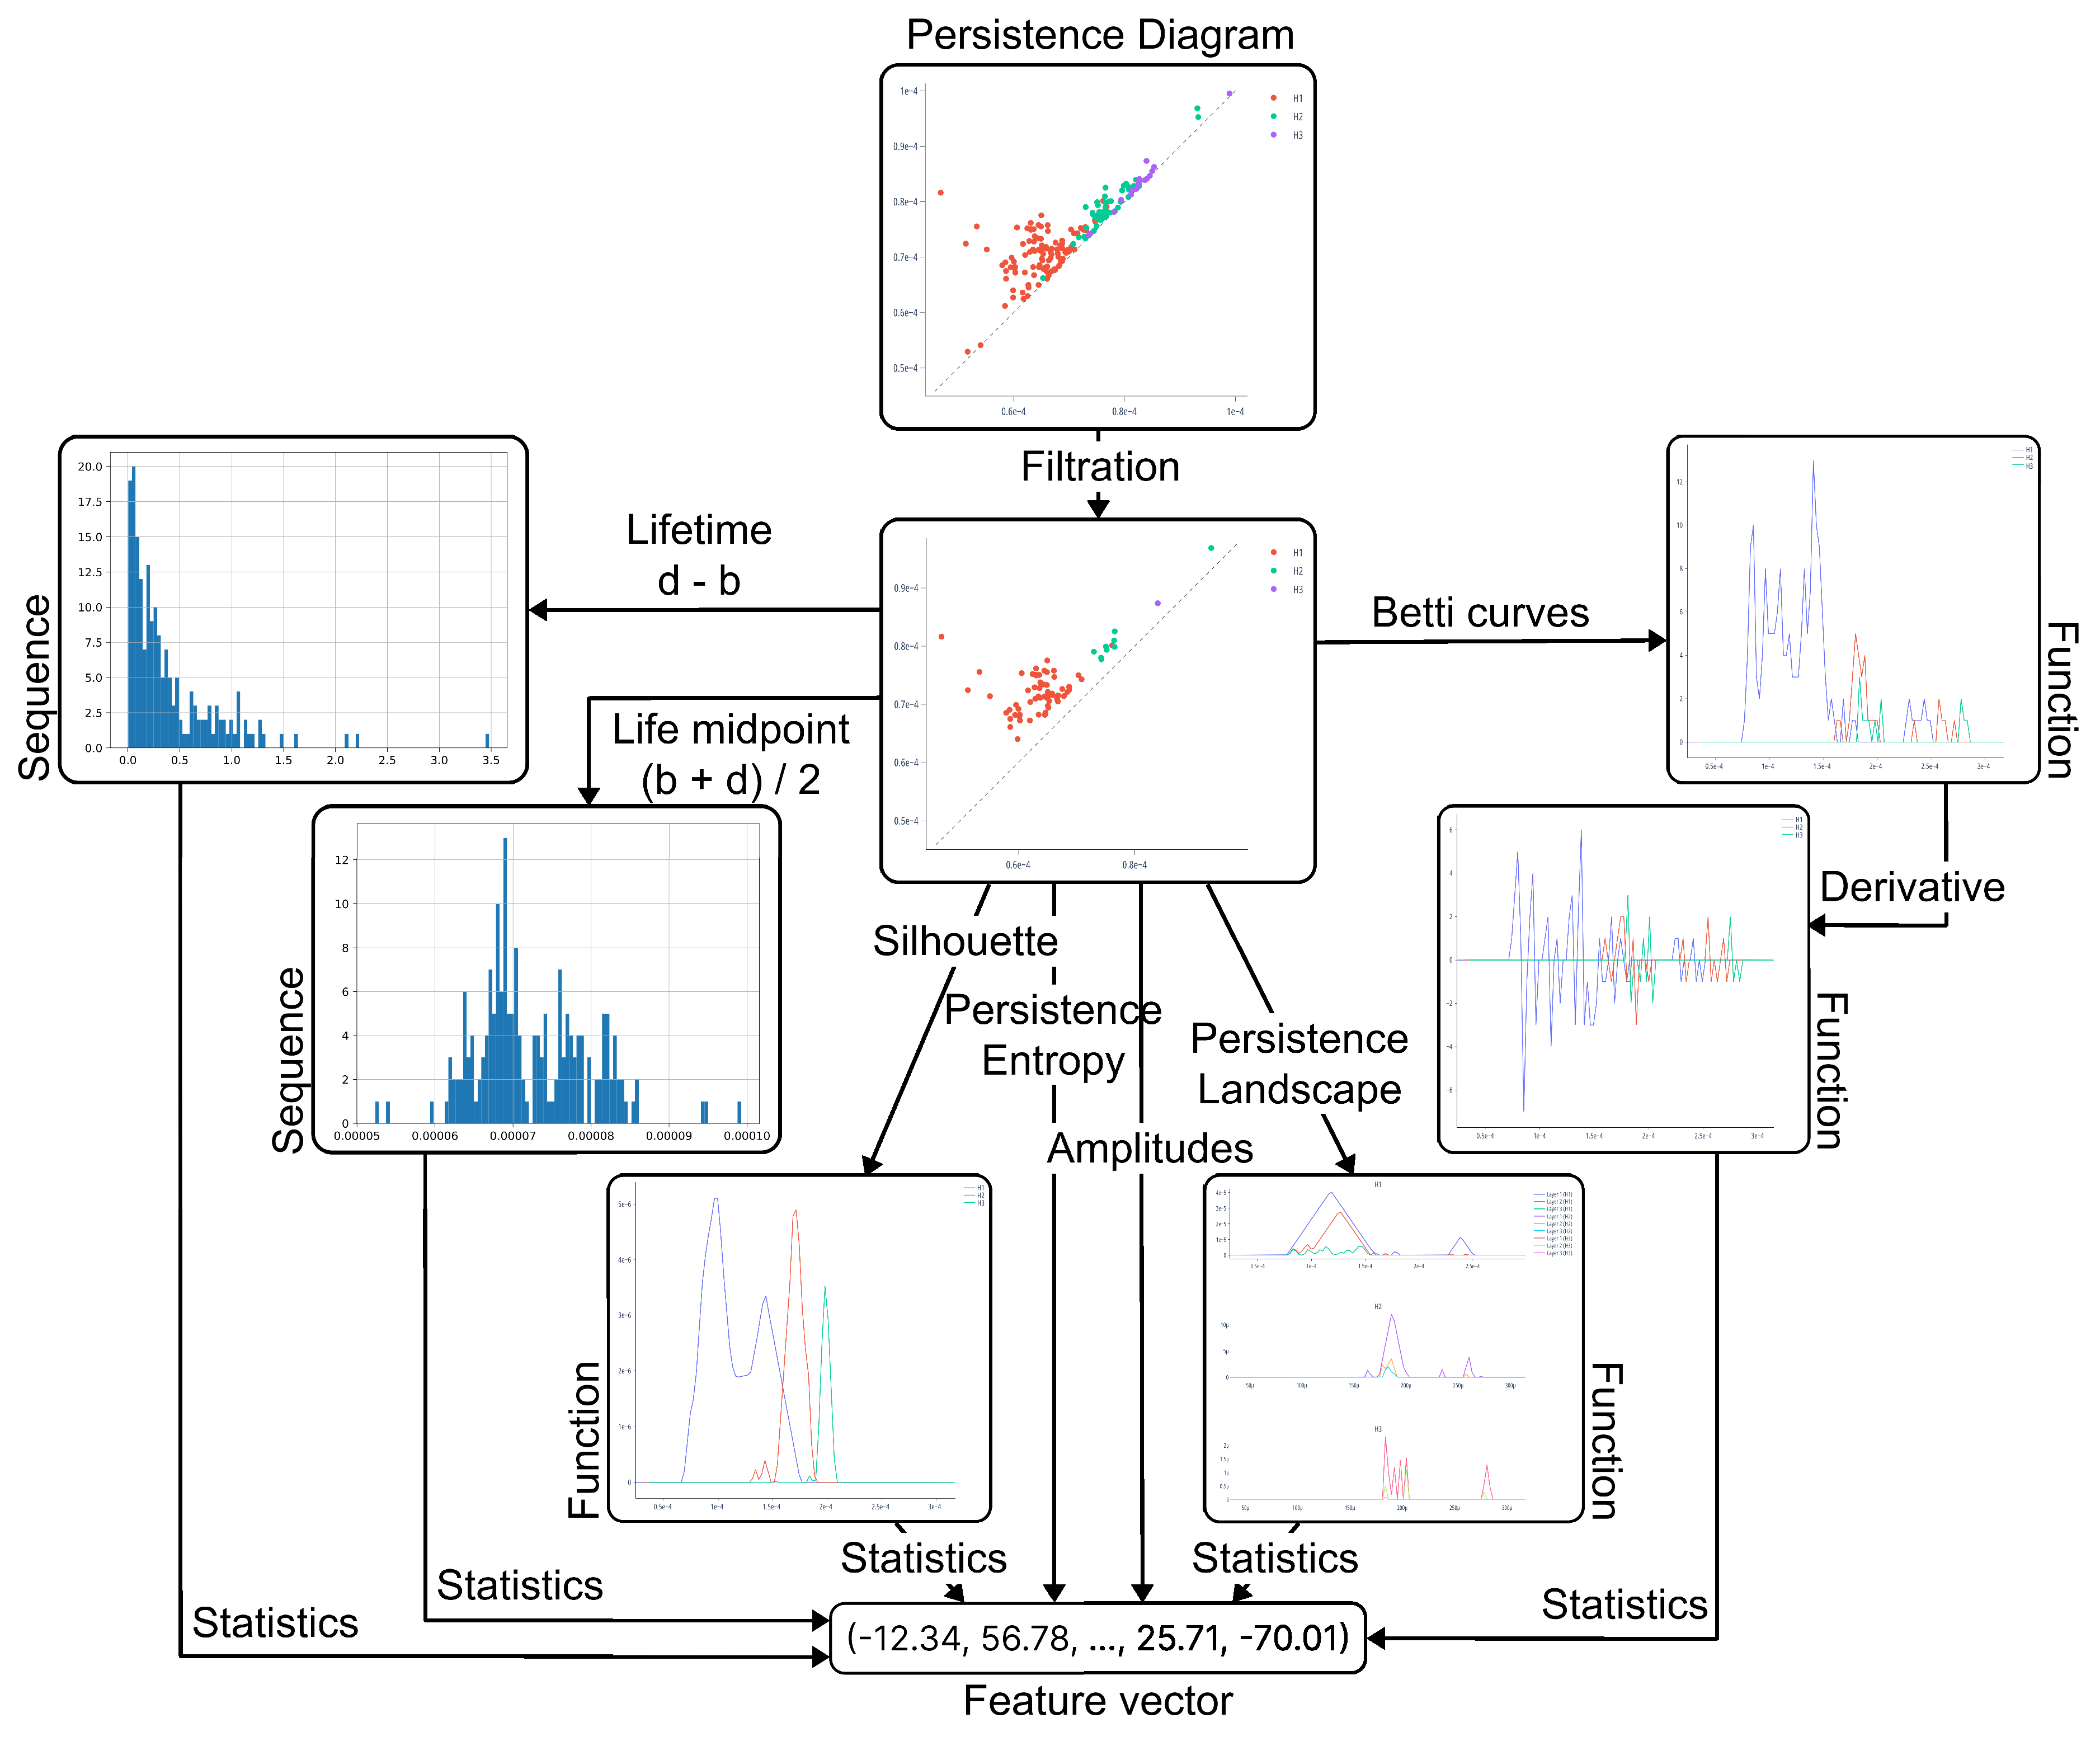
\includegraphics[width=\columnwidth]{figure4.eps}
    \caption{The scheme of the pipeline to vectorize the persistence diagrams.}
    \label{figure4}
\end{figure}

To improve the generalizing ability of the features, the algorithm begins by filtering the persistence diagrams --- removing a fixed fraction of the points closest to the diagonal, hence representing the simplices with the shortest lifetimes. These usually carry little information and most likely describe the `noise' ---  the patterns present in the original data but not generic among the objects of interest. The remaining points, in turn, are the most `long-lived' simplices that disappear significantly later than they appear and are generally most interesting for the analysis. 

The algorithm then calculates various topological and statistical characteristics described previously to construct a comprehensive feature description of the persistence diagram. That is, it computes the following values:
\begin{itemize}
    \item 
        The statistical characteristics of the sequences of lifetimes of simplices and of simplex life midpoints, of the first derivatives of Betti curves, of the first levels of persistence landscapes, and of the persistence silhouettes of degrees 1 and 2;
    \item 
        The persistence entropy;
    \item 
        The persistence amplitudes and their vector norms of first and second orders using the bottleneck distance, the Wasserstein distance, the Betti curves, the persistence landscapes, and the persistence silhouettes.
\end{itemize}

By the statistical characteristics of a numeric sequence or a function, that is, of a random variable, we suggest the following values:

\begin{itemize}
    \item 
        The quantity, maximum, sum, mean, standard deviation, and various percentiles (25th, 50th, and 75th) of the elements;
    \item 
        The Manhattan and Euclidean norms of the input as a vector;
    \item 
        The skew and kurtosis of the variable, that is, the ratio of the third and fourth central moments to the cube and the fourth power of the standard deviation, respectively.
\end{itemize}

To avoid missing significant patterns, we performed all calculations not only for the entire persistence diagram but also for each simplex dimension individually. When calculating the statistical characteristics of functions, we converted them into numeric sequences by selecting 100 values evenly over the interval of interest. Finally, we standardized all features to remove the scale factor from further decisions, which is known to improve the quality of most machine learning methods.

\subsection{Feature selection}

The feature engineering algorithm described earlier is designed to detect many patterns that may be present in the analyzed time series. However, this leads to extremely high dimensionality of the resulting vectors, which is undesirable for most machine-learning methods, including SDA, and may harm the quality of the final answer, especially if most assumed patterns are not present in the time series or appear insignificant to the target variable.

To address this issue, we introduce a quick state-detecting algorithm (QSDA) --- an additional step to select the most substantial features and filter out the noise that harms the final result. The algorithm operates as follows:
\begin{enumerate}
    \item 
        Calculate the possible final answers --- sets of state boundaries --- considering only one of the features by running a reduced SDA (that is, SDA with most hyperparameters adjusted to decrease the number of iterations, thus improving performance, without a significant loss in quality);
    \item
        For every produced set of edges, generate all possible ways to decrease the number of stages by merging the adjacent ones according to the rules provided by the SDA implementation;
    \item
        For every said way, calculate its quality as a function of the number of stages and the average silhouette coefficient against the considered feature over all pairs of adjacent stages;
    \item 
        Consider the maximum of the values obtained at the previous step as the quality score of the feature;
    \item
        Repeat the process for all features and select those with the highest quality scores as the most informative.
\end{enumerate}

Although steps (ii) and (iii) may seem ineffective and excessive, they are essential for the algorithm as we do not want to select features that poorly detect many stages over the ones that perfectly distinguish only a few. Furthermore, step (iii) allows for flexible adjustments to the importance of the detected number of stages compared to the silhouette coefficient. For this study, we used the multiple of the number of stages and the silhouette coefficient that demonstrated the best results compared to other tested possibilities.

One may also apply additional heuristics to remove the noisy, degenerate features, which are scored well solely because of the specifics of the approach. For example, consider a feature with just three non-zero values at indexes 300, 600, and 900 for the EEG of length 1200. Suppose at stages 1 -- 2 the algorithm calculated the boundaries $\{ 0, 280, 320, 580, 620, 880, 920, 1200 \}$, which results in a $0.74$ average silhouette and a $5.93$ final quality score of the feature, putting it above most non-degenerate ones at stage 5. Although the feature might contain some relevant information, it is evidently not valuable and will harm the final result. To counteract this, we preemptively filter out all features with less than 200 unique values --- about 20\% of the length of the analyzed EEG.\@

\subsection{Information value analysis}

Information value analysis~\cite{InformationValue} is a typical approach to evaluating the influence of individual features on the target variable in binary classification problems and can be natively generalized to assess the importance of features for clusterization.

Suppose $x=(x_1, x_2, \ldots, x_n)$ is a categorical feature with values from the set $\{ X_1, X_2, \ldots, X_k \}$ and $y=(y_1, y_2, \ldots, y_n)$ is a binary target variable. Then, for each value $X_i$, the weight of evidence is calculated using equation \eref{eq2} as the ratio of the shares of positive and negative objects with this value of the feature. Finally, the information value of this feature is computed using equation \eref{eq3} and is an estimate of how much the distribution of this feature coincides with the distribution of the target variable, thus showing how important this feature is for the correct classification of objects.
\begin{eqnarray}
    sharePos_i = numPos_i / numPos, \nonumber\\
    shareNeg_i = numNeg_i / numNeg, \nonumber\\
    WoE_i = shareEvents_i / shareNonEvents_i, \label{eq2}\\
    IV = \sum_{i = 1}^{k} (sharePos_i - shareNeg_i) \cdot WoE_i, \label{eq3}
\end{eqnarray}

with:
\begin{itemize}
    \item
        $numPos_i$ and $numNeg_i$ the number of objects belonging to the positive and negative classes, respectively, whose value of the feature is $X_i$;
    \item
        $numPos$ and $numNeg$ the total number of objects belonging to the positive and negative classes, respectively;
\end{itemize}

When working with quantitative features, the values are divided into several containers (we used 10) of the same length and processed as categorical based on their belonging to one or another container. For a multi-class classification problem, the information value is calculated independently for each class relative to a binary indicator variable with subsequent averaging of the values. The clusterization task is considered similarly, with each cluster treated as a separate class.

Large values of the information value correspond to the high generalizing ability of the feature and its significant influence on the correct prediction of the target variable. On the other hand, values close to zero indicate the harmfulness of the feature when making predictions.

\section{Results}

To analyze the applicability of topological data analysis to finding the hidden functional states from EEG, we compared the results obtained using different types of features: 765 traditional features from~\cite{SDA}, 1500 -- 2000 topological features selected with qSDA, and the feature space with both approaches combined. The hyperparameters were mostly deduced experimentally using the EEG of object 1, which is the shortest recording yet exhibits the most well-defined stage boundaries. Finally, we analyzed the information values of all topological features relative to the result they produced and compared them with the scores and best features calculated using qSDA.\@ To reinforce the statistical significance of our conclusions, we repeated the analysis for EEG recordings obtained from the original ones by randomly shuffling the epochs, expecting to detect no good stage boundaries resulting in close-to-zero quality metrics.

\subsection{Objects~1 3}

Based on our experiments shown in \fref{figure5}, the most stable and performant dimensionality reduction technique is the PCA, which we thus used further throughout the experiment to reduce the feature spaces to 15 components  to improve comparability and filter out the noise, capturing only the most significant patterns. The features generated by UMAP demonstrate good clusterization quality independent of the number of components for all subjects but have relatively low explained variance, which massively hinders their interpretability. On the other hand, the traditional autoencoder reflects the original feature space well and demonstrates quality similar to PCA.\@ However, for further calculations, as mentioned previously, we selected the latter, more deterministic approach to speed up the computations and facilitate comparison with the original paper's results. Interestingly, the topological autoencoder produces mostly meaningless embeddings and has low explained variance while also achieving the worst results among all methods. 

\begin{figure}
    \centering
    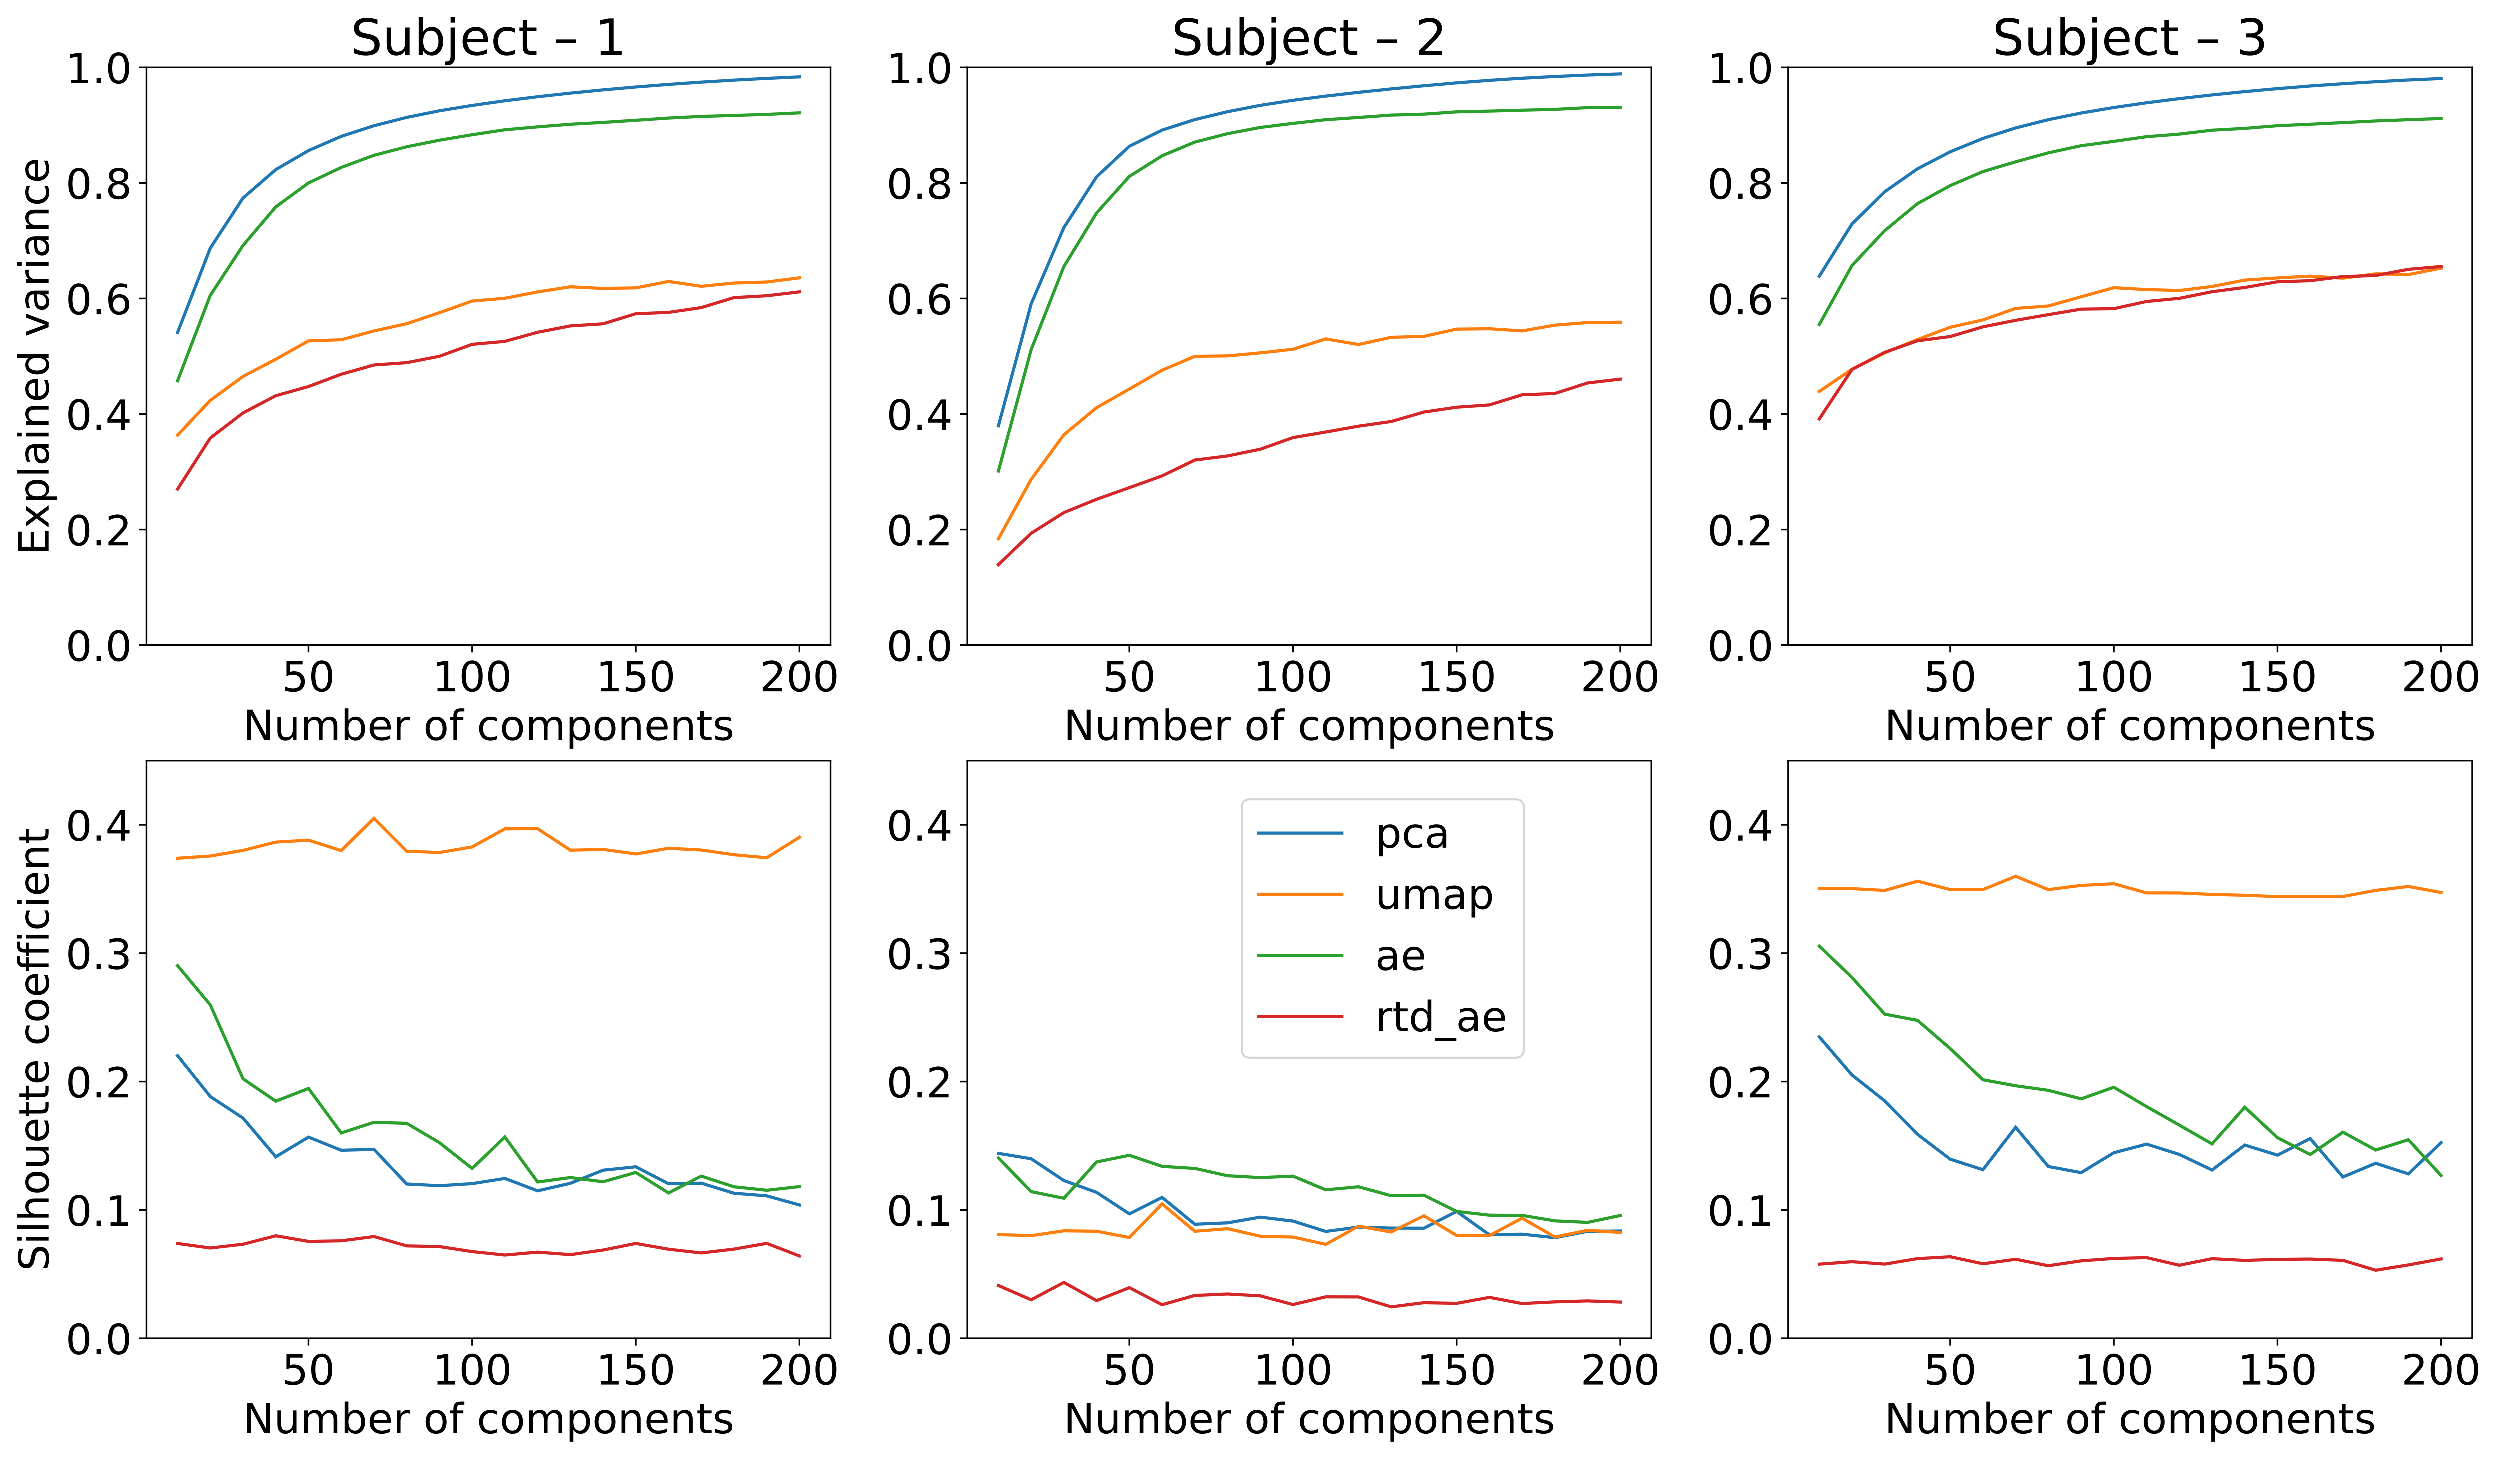
\includegraphics[width=\columnwidth]{figure5.eps}
    \caption{
        Explained variance (top) and achieved resulting quality (bottom) of four dimensionality reduction algorithms for objects 1 (left), 2 (middle), and 3 (right).
    }
    \label{figure5}
\end{figure}

As illustrated in \fref{figure6}, topological features demonstrate results comparable to traditional ones, with some stage boundaries almost precisely matching for all types of features throughout all objects. Furthermore, according to \tref{table1}, topological features outperform the traditional ones for all experiments, with the combined feature space achieving an even higher silhouette score for object 1, although following slightly behind for objects 2 and 3. 

However, the scatter plots in \fref{figure6} show noticeably higher density and better separation of the stage\mbox{-}2 boundary candidates when the spectral features are involved. This indicates higher stability of the final results obtained in those cases, except, arguably, for object 2, where the illustrations are insufficient to make conclusive decisions. Nevertheless, in all cases, SDA did not discover any meaningful patterns when applied to shuffled recordings and demonstrated over 10 times lower quality than for the original data, reinforcing the statistical significance of the results.

\Table{
    \label{table1}
    Silhouette coefficients of results obtained from original and shuffled recordings of all objects using three sets of features: traditional, topological, and combined.
}
    \br
    EEG recording & Traditional & Topological & Combined\\
    \mr
    Object 1 (original) & 0.198 & 0.205 & 0.218 \\
    Object 1 (shuffled) & 0.004 & 0.008 & 0.005 \\ \bs
    Object 2 (original) & 0.110 & 0.131 & 0.126 \\
    Object 2 (shuffled) & 0.008 & 0.006 & 0.009 \\ \bs
    Object 3 (original) & 0.111 & 0.190 & 0.187 \\
    Object 3 (shuffled) & 0.017 & 0.005 & 0.004 \\
    \br
\endTable

\begin{figure}
    \centering
    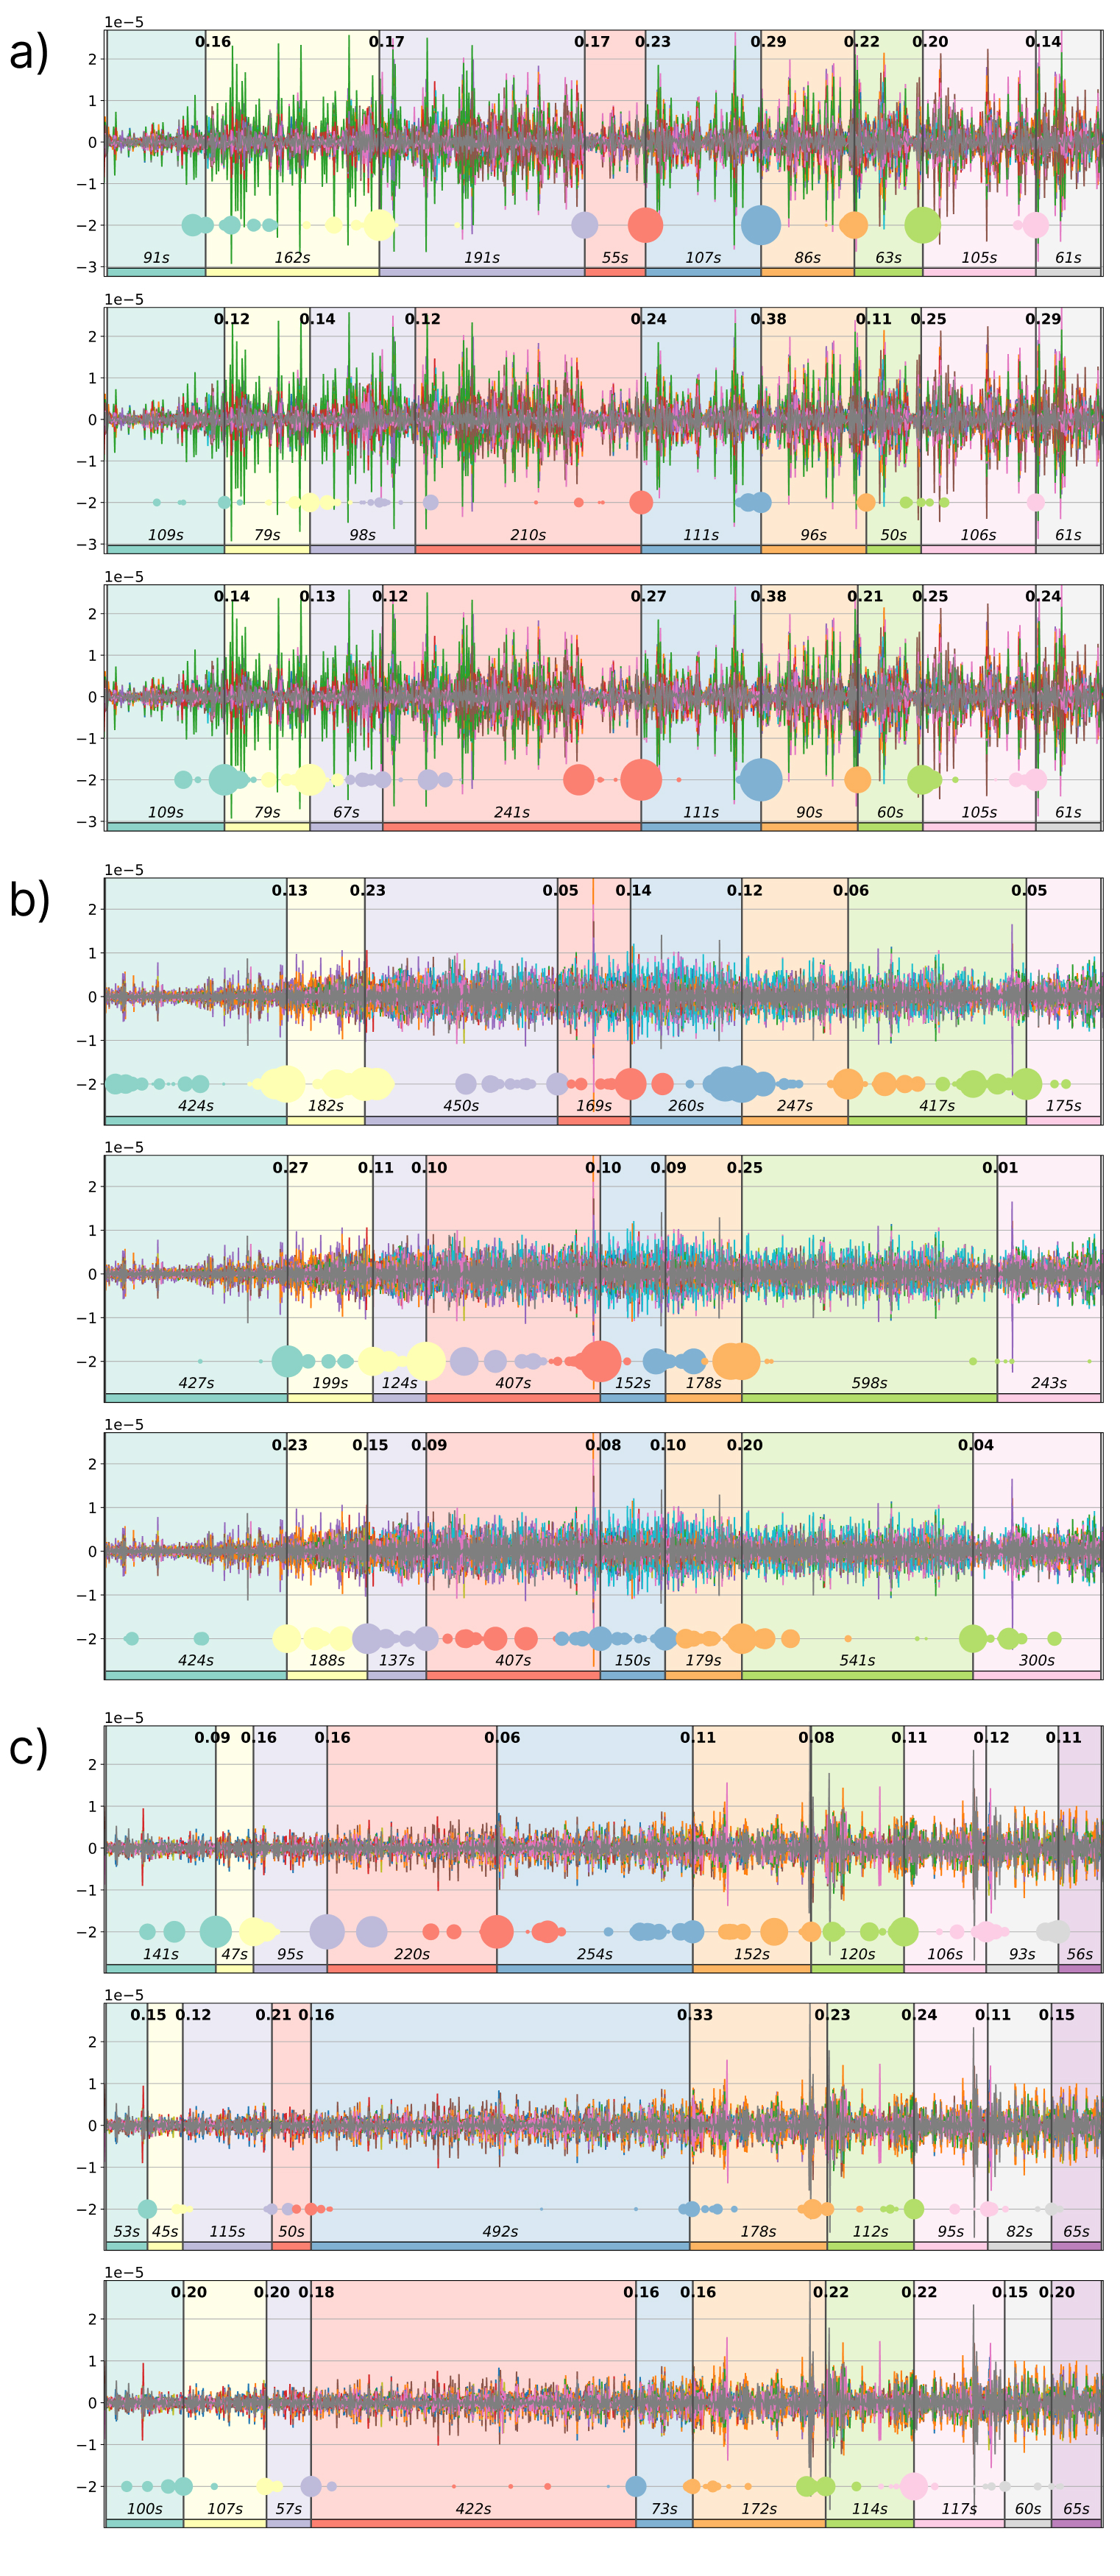
\includegraphics[width=0.95 \columnwidth]{figure6.jpeg}
    \caption{Original EEG recordings of objects 1 (a), 2 (b), and 3 (c) with detected stages outlined in different colors and their durations indicated at the bottoms of the diagrams. Top charts display results obtained using traditional features, middle charts --- using topological ones, and bottom charts --- using both approaches together. Vertical black lines are the final state boundaries computed by SDA as the centers of corresponding clusters shown on multicolored scatter plots at the bottom of each chart. The scatter plots represent the joint arrays of state boundary candidates obtained in the second step of SDA, with the dot size reflecting the frequency of occurrence of an epoch in this array and illustrating the stability of the boundary. The black numbers at the top of each chart present the silhouette coefficients for pairs of adjacent stages of each discovered boundary.}
    \label{figure6}
\end{figure}

Overall, SDA successfully identified well-separated functional stages in all three EEG recordings with all considered feature spaces. Although we did not achieve a complete agreement between the results, one can undoubtedly trace the common patterns confirmed by relatively good values of quality metrics for all objects. Furthermore, the topological approach led to better partitions according to the silhouette coefficient for all monks, although the traditional techniques usually prevailed in the stability of the answers. However, when using the novel approach, the algorithm significantly shifted or did not determine the individual boundaries separating similar states with low intercluster distances, which may indicate both that topological features lose important patterns present in the original data and that they reveal additional significant dependencies not recorded by the spectral features. Accounting for the results with the combined feature space, we suggest that the topological features most likely do not duplicate but complement the traditional ones to achieve even better, stable results. Our experiments show that they may miss some critical patterns but discover other unexplored ones, which is reinforced by the combined features demonstrating comparable or exceeding quality than other approaches while having higher stability. Finally, the statistical significance of the results is reinforced by the extremely low quality obtained using shuffled recordings.

As shown in \fref{figure7}, the most informative features consistently across QSDA and information value analysis for all objects were various persistence amplitudes. Interestingly, unlike IV, QSDA especially preferred the ones based on persistence silhouettes and landscapes while massively underestimating those calculated from betti curves. However, the assessment techniques did not highlight any evident brain regions producing the most valuable features across all three objects. Nonetheless, the scores are generally consistent between the feature selection methods. For object 1, both strategies valued recordings obtained from the right and occipital parts of the brain, for object 2 --- from the prefrontal, frontal, and midline areas, and for object 3 --- from the temporal and frontal brain regions. Notably, QSDA generally shifted its preference towards the occipital and parietal parts, although the principal trends persisted. Regardless, both approaches consistently scored the features resulting from Pearson dissimilarities low. Aggregated by the topological origin, although the simplices of dimensions 1 and 2 contributed the most, the best features were those describing all dimensions simultaneously, suggesting that higher dimensions do not duplicate but rather complement the patterns detected by simpler features. Interestingly, for object 2, QSDA also favored the simplices of dimension 5 --- the pattern not observed in other cases. Finally, the most meaningful statistical characteristics were the vector norms with $p = 1$ and $p = 2$, as well as the sum and mean of the input. The least informative, in turn, were all percentiles (25, 50, and 75), skew, and kurtosis of the variables.

\begin{figure}
    \centering
    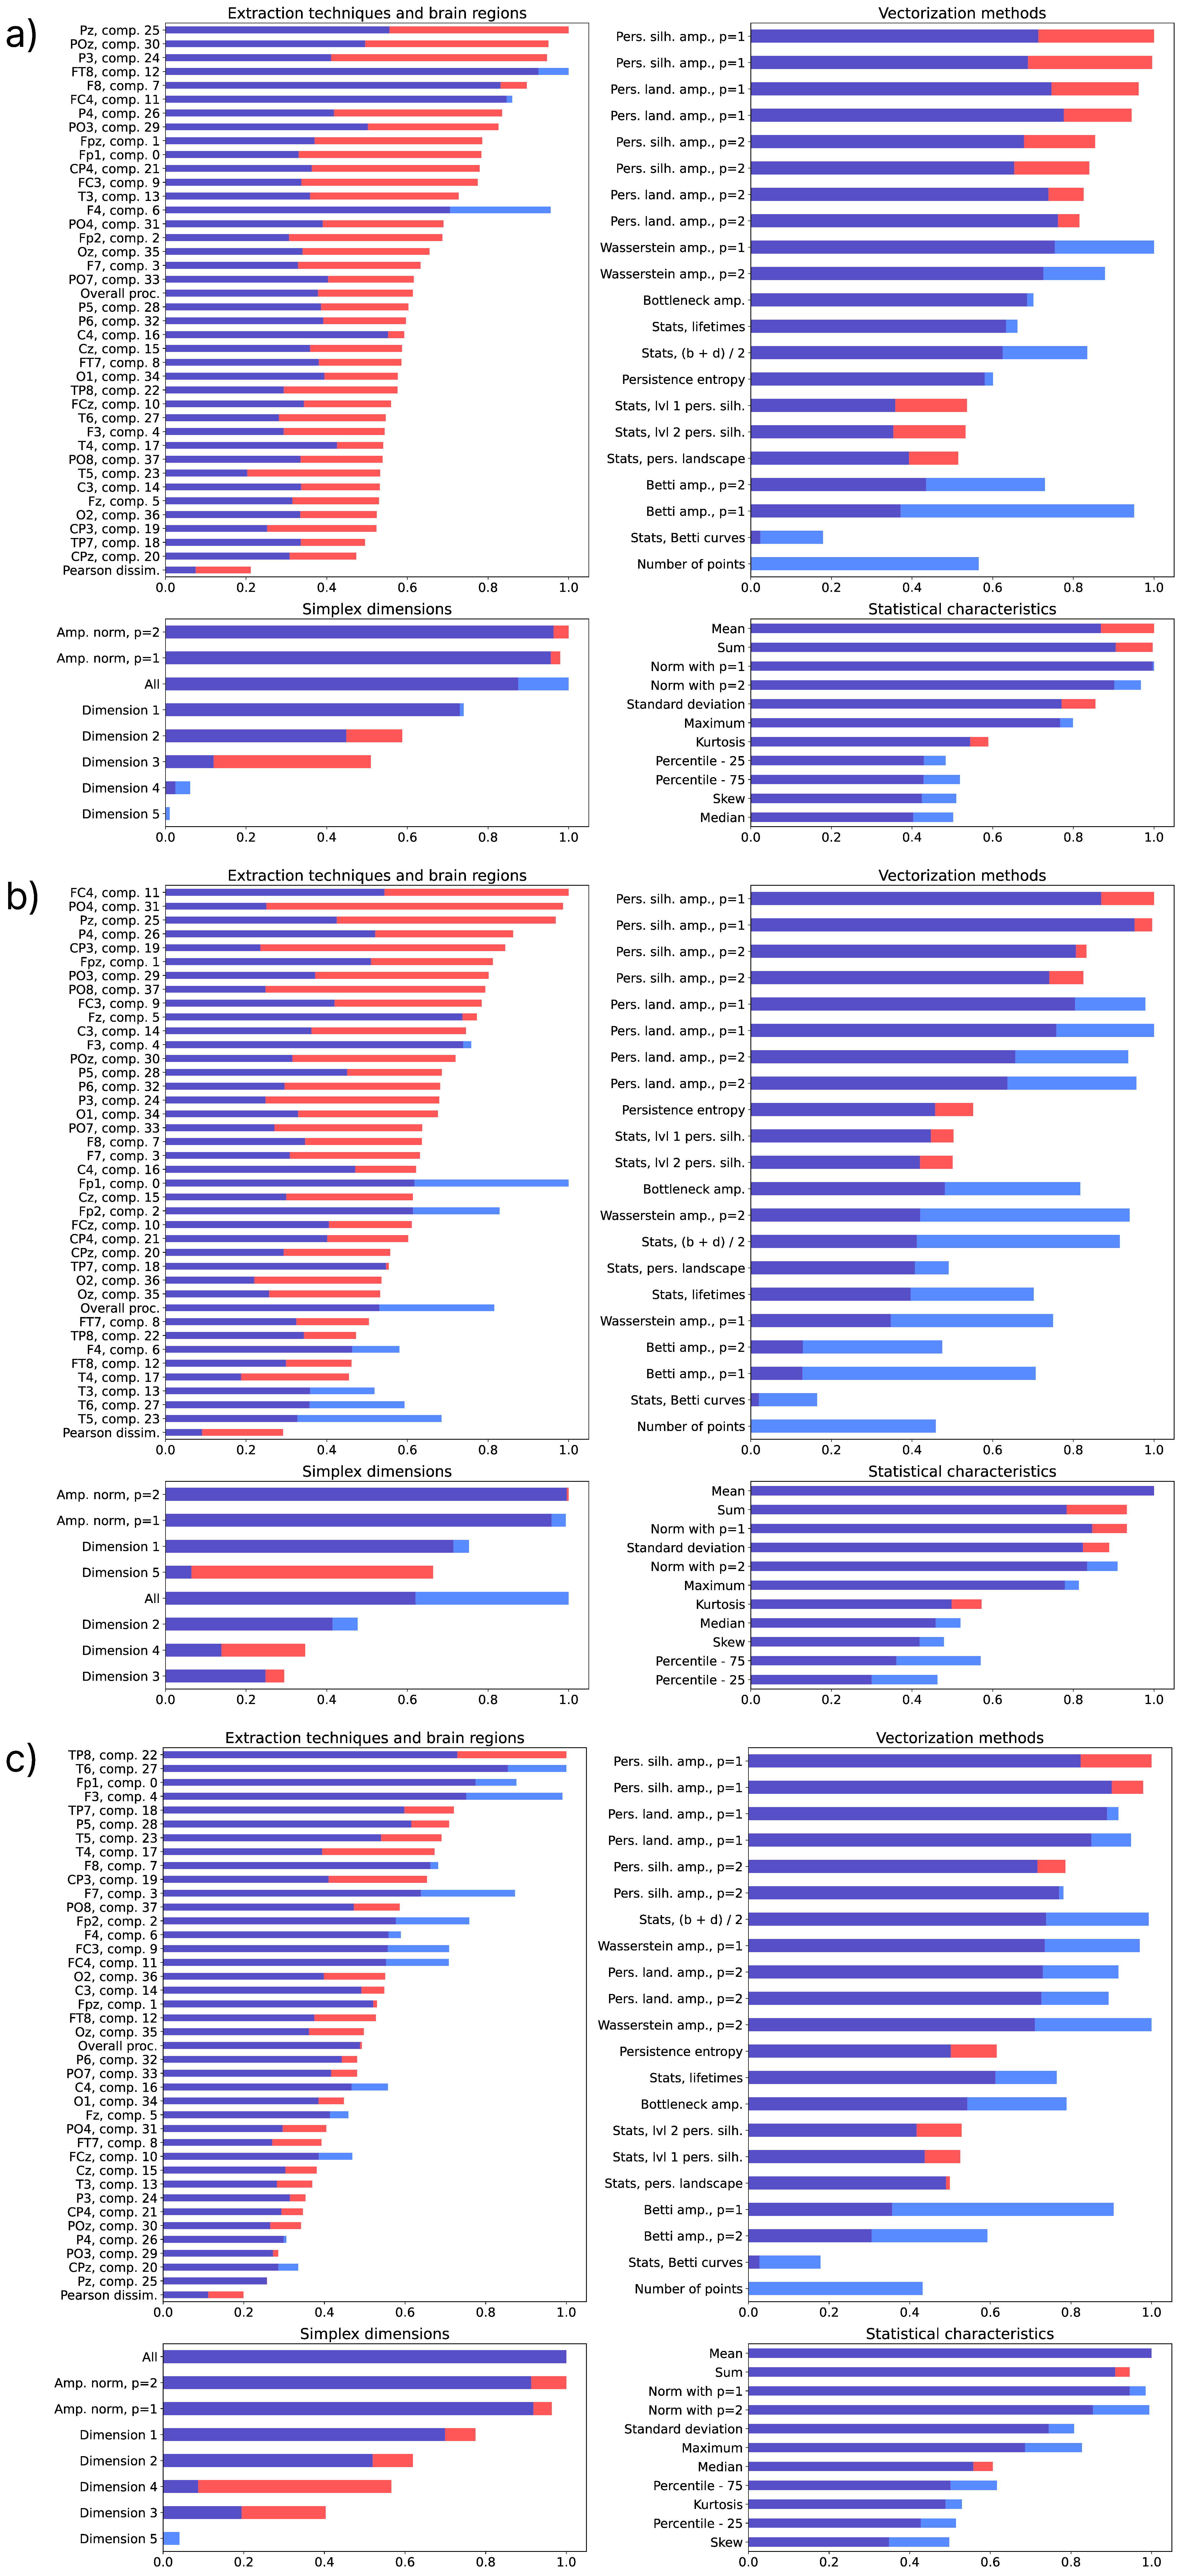
\includegraphics[width=\columnwidth]{figure7.eps}
    \caption{Mean information values (blue) and QSDA scores (red) of all topological features for objects 1 (a), 2 (b), and 3 (c), aggregated by the parameters of their source: extraction technique and brain region (top left), vectorization method (top right), simplex dimension (bottom left), and statistical characteristic (bottom right).}
    \label{figure7}
\end{figure}

% This is here to force placement on the same page with the describing text in a two-column layout
\begin{figure*}
    \centering
    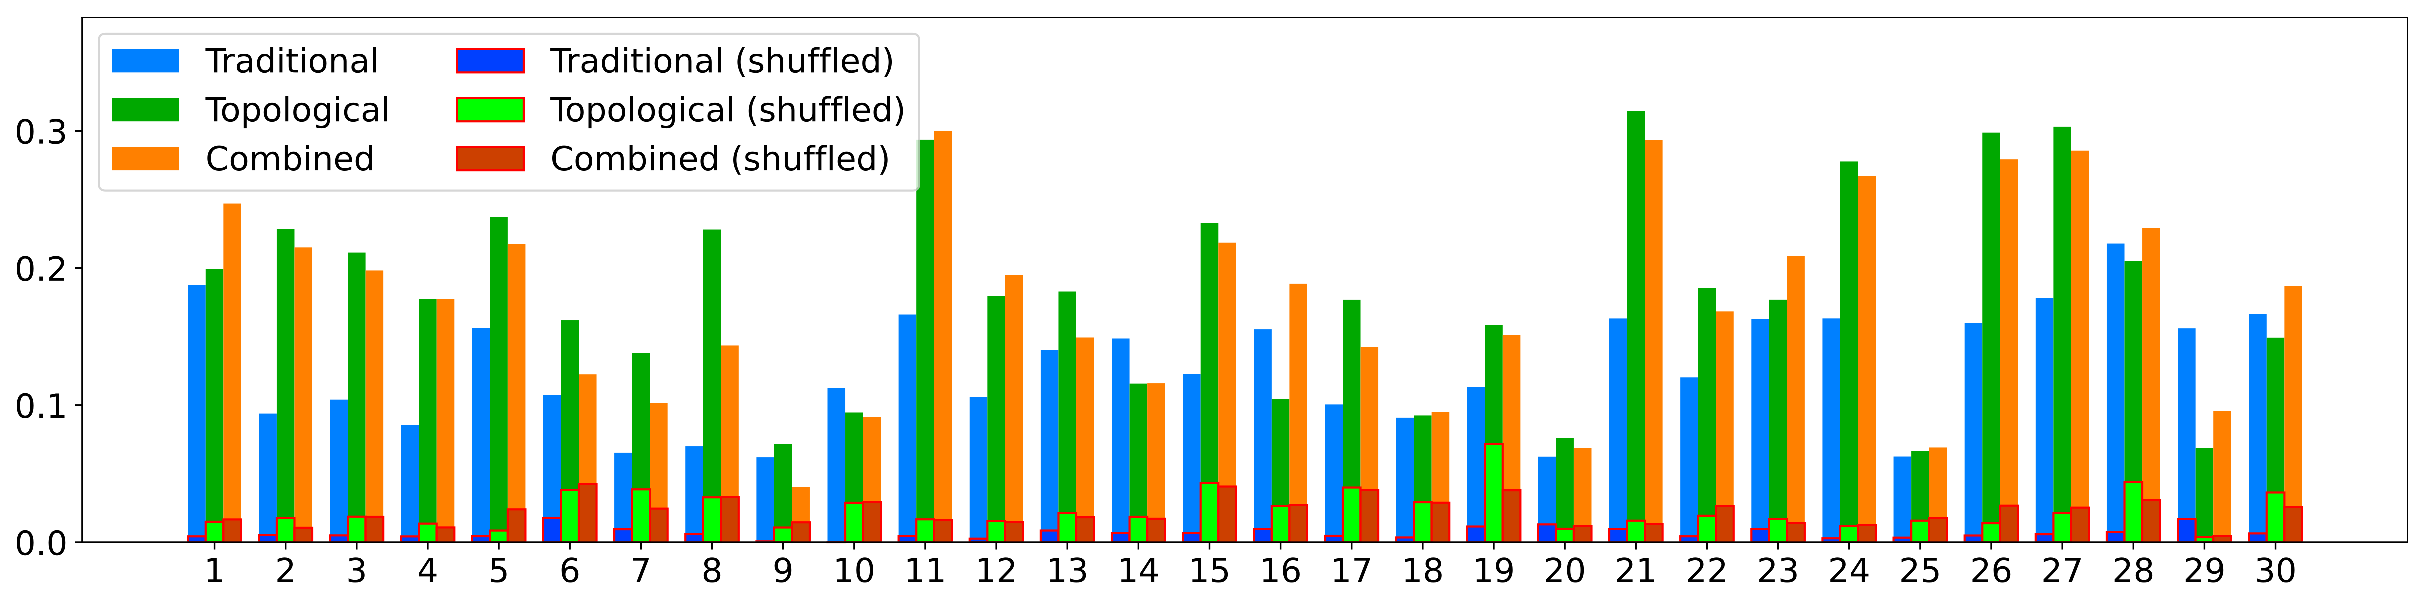
\includegraphics[width=\textwidth]{figure8.eps}
    \caption{The silhouette scores of the resulting boundaries deduced by SDA using three types of features for the original and shuffled recordings of 30 subjects.}
    \label{figure8}
\end{figure*}

It is worth noting that the extremely high dimensionality of the topological features might have introduced some dispersion in the results. However, the proposed selection method (QSDA) demonstrated effectiveness in filtering out significant portions of noisy features and was supported by the information value analysis. Although one may notice some discrepancies in its behavior compared to IV (for example, giving preference to the data collected closer to the occipital part of the brain and overestimating the quality of some amplitudes), the principal patterns match for both approaches.

\subsection{Validation with 30 objects}

To reinforce our results, we additionally run the proposed algorithm on the EEG recordings of the Buddhist Tantric Guhyasamaja meditation practice performed by 30 more Tibetan monks. To enhance the stability of the detected stages and to speed up the computations, we removed the features that established ineffective for the recordings already analyzed, that is:
\begin{itemize}
    \item 
        All features computed from Pearson dissimilarities between the components of the EEG;\@
    \item 
        The features resulting from Betti curves and the numbers of points on the persistence diagrams, including the respective amplitudes;
    \item 
        The percentiles, skew, and kurtosis of the variables.
\end{itemize}

As a result, we obtained around 4,500 topological features (as opposed to 20,000 previously), from which we selected the 25\% best ones using QSDA.\@

As shown in Figure 8, the topological features outperformed the traditional ones for most subjects, while the combined feature spaces were prevalent for a third of the recordings. Furthermore, the scores on shuffled epochs were multiple times lower than the ones for the original EEG recordings and did not exceed 0.05 for all subjects. Thus, no evident good patterns have been detected for shuffled epochs, reinforcing the statistical significance of the results.

Finally, these experiments provide sufficient evidence to argue that the most valuable data for the research generally comes from the electrodes in the frontal area of the brain, with the sensors Fp1, Fp2, and F7 proving the most applicable information, as strongly supported by both the aggregated QSDA (\fref{figure9}, left) and IV (\fref{figure9}, right) quality scores.

\begin{figure}
    \centering
    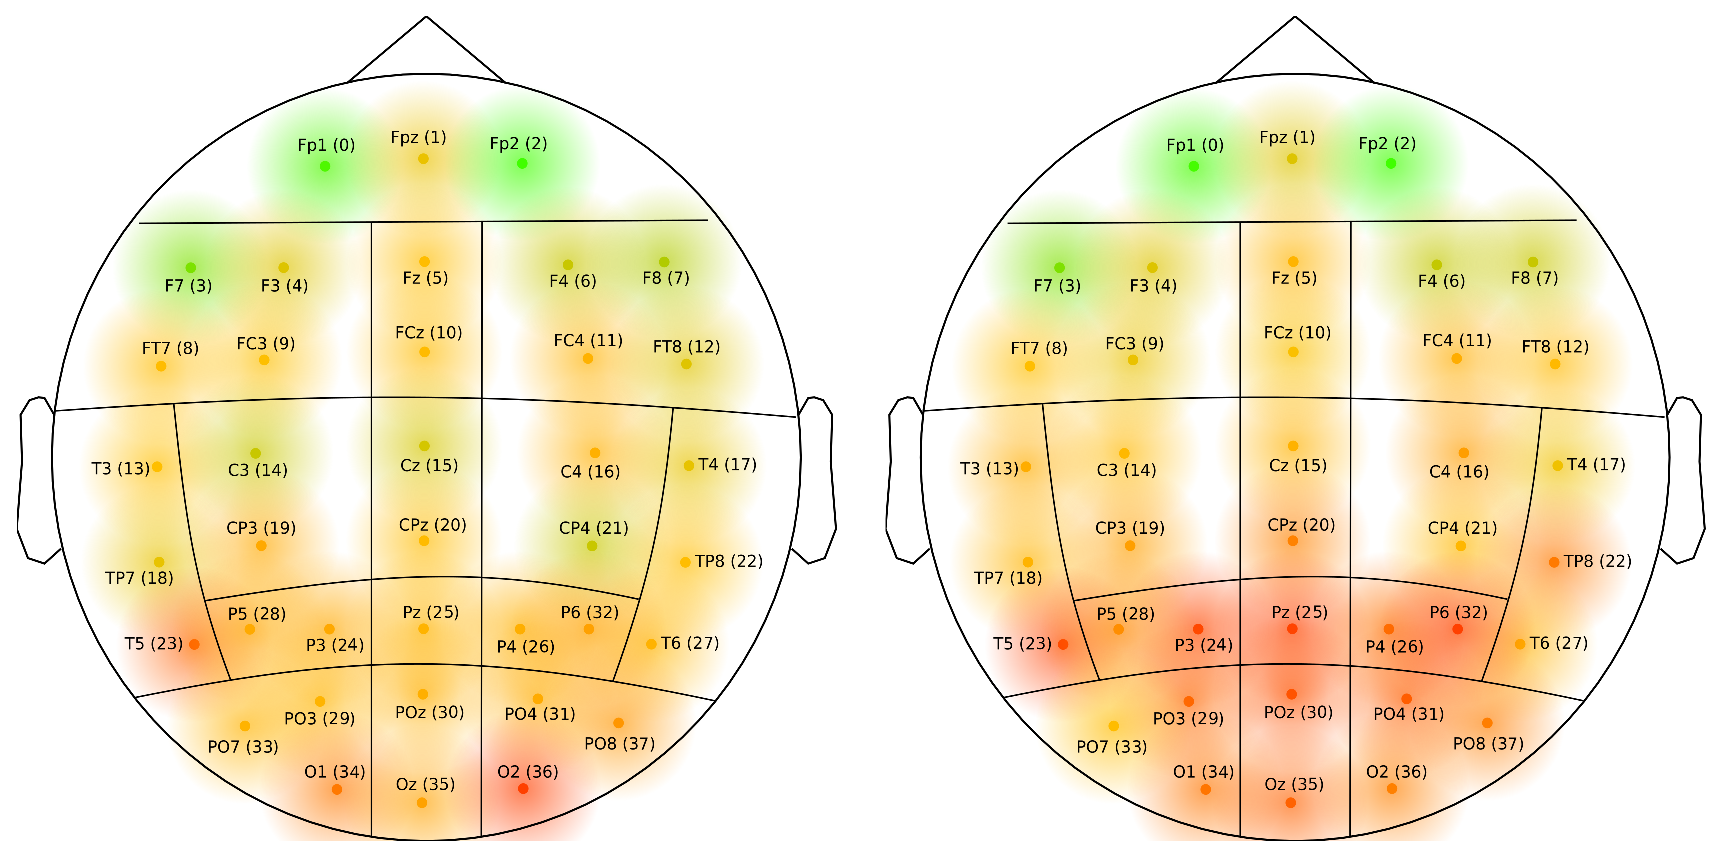
\includegraphics[width=\columnwidth]{figure9.eps}
    \caption{Feature quality scores (QSDA on the left, IV on the right) aggregated by their source electrode averaged over 30 subjects.}
    \label{figure9}
\end{figure}

\section{Conslusions and discussion}

In this study, we combined various topological methods and proposed an algorithm to construct a comprehensive feature description of the time series, which proved effective in finding the functional stages in the EEG recordings of the Guhyasamaja meditation practice performed by 30 Buddhist monks. As demonstrated by the experiment, with proper feature engineering, the SDA --- a novel automated approach to solving the task --- can find boundaries similar to the ones obtained previously using solely the traditional features. However, in some cases, the technique preferred less similar results, which indicates both the loss of important information in the process of topological analysis and the discovery of new patterns previously not identified by existing solutions.

Based on our research of the separate and combined behavior of the traditional and topological features, we suggest that neither approach extracts a complete description of the EEG.\@ Although there are certain intersections, the topological and spectral characteristics mostly describe distinct dependencies in the data, complementing each other, emphasizing the known patterns, and discovering new ones. Thus, there is no silver bullet to solving the task, but one should combine the approaches to achieve a stable result that reflects the actual behavior of the studied process.

Additionally, SDA detected no significant stage boundaries when applied to the shuffled epochs, demonstrating several times lower quality metrics compared to the original EEG for all analyzed objects. Thus, we consider the obtained results reliable and suggest that the topological approach produces good features that do not hinder the stability of SDA.\@

Finally, we introduced a novel, SDA-based feature selection framework that proved effective in removing the noisy features that are detrimental to good clusterization of the EEG.\@ The algorithm's scores primarily correlate with the information values of the features, which confirms its results and reinforces the rationality of using the alleged best features to solve the problem at hand.

Future studies should test the proposed approach with other data sets to generalize the technique and identify common patterns. We expect especially intriguing results when applied to well-studied data with known correct placement of functional state boundaries. Moreover, we expect significant outcomes from studies aiming to interpret the patterns recorded by topological features accounting for the structure and patterns authentically observed in the original data.

\section*{Data availability statement}

The raw data will be made available by the authors upon request, without undue reservation.

\section*{Declaration of conflicting interest}

The author(s) declared no potential conflicts of interest with respect to the research, authorship, and/or publication of this article.

\section*{References}

\bibliography{references}{}
\bibliographystyle{iopart-num}

\end{document}
